\subsection{Measurement}

In this section, I will first discuss measurement issues. And then within each research design section I will specifically discuss data availability and which measurement is available.

\subsubsection{Measuring spillover}

Since detecting spillover effect is itself a major research program, my research will get at this from multiple angles. First, I will measure spillover indirectly with two theoretically driven measures: 1) the \% of private firms engaging in business relations with foreign firms, and 2) the \% of private firms that exports

We can also measure spillover directly. This is done in two steps.

First, measure the level of technology or productivity of a firm.

Level of technology: 

Level of productivity: Consider the familiar Cobb-Douglas production function:

\begin{align}
Y &= AL^{\alpha}K^{\beta}
\end{align}

where $Y$ is value added, $A$ is total-factor productivity (TFP), $L$ is labor, and $K$ is capital. $y$, $L$, and $K$ are observable, while $A$ is not. Log transform both sides of the equation, we attain a linear form:

\begin{align} \label{eq:cobb_douglas_linear}
y &= a + \alpha l + \beta k
\end{align}

where the lowercase variables are the log-form of the uppercase variables (e.g. $y = \log(Y)$ and so on). \autoref{eq:cobb_douglas_linear} can then be estimated with OLS:

\begin{align} \label{eq:cobb_douglas_OLS}
y_i = \beta_0 + \beta_1 l_i + \beta_2 k_i + \epsilon_i
\end{align} 

where $\beta_0$ is the average total-factor productivity of all firms and $\epsilon$ is the firm-specific deviation from that mean. From the estimated coefficients of \autoref{eq:cobb_douglas_OLS}, we can estimate firm-level total-factor productivity as follows:

\begin{align}
a_i &= \hat\beta_0 + \hat\epsilon_i \\
A &= \exp^{\hat\beta_0 + \hat\epsilon_i}
\end{align}

Having estimated firm-level TFP and technology, we then regress TFP (technology) on the presence of FDI in a country (sector). FDI presence can be measured as:
\begin{itemize}
\item amount of FDI
\item number of foreign firms in a country (sector)
\item number of foreign firms that the domestic firms are in contact with (for forward and backward linkage)
\end{itemize}

\subsection{Hierarchical model using cross-national, cross-sectoral data}

Also measure directly: Doing Business questions on capacity and innovation. Then regress innovation on FDI presence

(which DB has data on the number of suppliers/customers that are foreign. We can perhaps divide this by the total number of suppliers and customers)

TFP (total factor productivity) = residuals of regressing value added on capital and labor input (DB has total asset (capital), total value of sale, total value of material + fuel, number of workers)

To measure corruption, presence of FDI, and treatment of firms across countries, I utilize the World Bank's Enterprise Survey (ES), which includes a wealth of firm-level data across 125 countries, spanning various topics from investment, labor, to business-government relation \citep{WorldBank2015}. The Enterprise Survey uses stratified random sampling (using three strata: firm size, business sector, and region) in order to ensure representativeness. The survey data comes from face-to-face interviews with upper management and is anonymized to ensure confidentiality at all times.\footnote{For more on the methodology of the Enterprise Survey, visit \url{http://www.enterprisesurveys.org/methodology}} This dataset has a wealth of firm-level data that helps us operationalize key concepts as detailed below.

Recall our hypothesis:

\begin{quote}
Hypothesis: The presence of large FDI firms in corrupt countries is associated with a large gap in the government's treatment of domestic firms and foreign firms in those countries.
\end{quote}

\begin{quote}
Hypothesis: The presence of large FDI firms in corrupt sectors is associated with a large gap in the government's treatment of domestic firms and foreign firms in those sectors.
\end{quote}

Operationalization of independent variables:
\begin{itemize}
\item FDI in countries: available via UNCTAD data on FDI flows and stocks to countries.

\item FDI in sectors: available via the Enterprises Survey dataset. The ``largeness'' of FDI firms can be measured by constructing a Herfindahl-Hirschman Index based on the size of sale, labor, or capital of firms. This allows us to calibrate the ``largeness'' of FDI firms according to the size of the host country's market.

\item Corruption: can be measured in two ways. 1) Firms' perception about corruption as an obstacle. This measure is frequently used but not accurate since firms' perception of corruption depends not only on the level of corruption but also the characteristics of firms. 2) Hard measure of prevalence and depth of bribes, e.g. ``Was an informal payment expected or request (when applying for a license)?'', ``How much do establishments like this one give in informal payments?'' 
\end{itemize}

Operationalization of dependent variable (i.e. the gap in the government's treatment of domestic firms and foreign firms):
\begin{itemize}
\item The gap can be measured by hard measures of business experience. It is important to choose aspects of the business experience that can be \textit{selectively} targeted by the government, e.g. tax rate, time spent dealing with inspectors, etc. In contrast, other aspects, such as quality of the labor force, days without electricity, etc. are harder to be targeted to a certain type of firms. These aspects can serve as the dependent variables in a placebo test.

It is important to note that this design does not suffer from selection bias. In the large literature using FDI survey data, it is impossible to control for the fact that the foreign firms that show up in the sample are the ones that self-select into investing. However, this is not an issue for our design. Because foreign firms that self-select into investing are more likely to be similar to domestic firms than foreign firms that do not, the \textit{observed} gap in the business experience of foreign and domestic firms in the sample is biased downwards and against our hypothesis.
\end{itemize}

\subsection{Cross-sectoral and sub-national variation in Vietnam}

As mentioned earlier, despite the wealth of firm-level, cross-national data in the ES dataset, its measure of corruption is still plagued by a host of measurement issues. Asking directly about firms' experience with corruption is unlikely to get an accurate answer due to sensitivity bias \citep{Coutts2011}. Researchers, including the ES team, often address this problem by framing the question about the experience with corruption of ``firms like yours.'' However, with this technique, firms may not read between the lines and actually answer about the experience of others \citep{Ahart2004}.

I remedy these problems with a research design focusing on the case of Vietnam, taking advantage by a survey list experiment by \citet{Malesky2015}, which uses unmatched count technique to accurately measure the experience of firms with corruption while avoiding sensitivity bias.

Recall the hypothesis:

\begin{quote}
Hypothesis: The presence of large FDI firms in provinces whose leaders are not interested in promotion is associated with a large gap in the government's treatment of domestic and foreign firms.
\end{quote}

Operationalization of independent variables:
\begin{itemize}
\item FDI in province: provincial statistics of FDI flow (government website)
\item FDI in sectors: government website
\item Corruption: list experiment \citep{Malesky2015}
\item Interest in promotion: 
\begin{itemize}
	\item base chance of promotion: years until retirement (retirement age is 60 for male, 55 for female)
	\item appearance in centrally controlled newspapers as a proxy for the decision to pursue promotion
\end{itemize}
\end{itemize}

Operationalization of the dependent variable, i.e. the gap in the government's treatment of the foreign and domestic firms
\begin{itemize}
	\item PCI survey question: ``Do you think that the provincial officials prefer FDI?'' (Question H3)
	\item The gap in the perception of domestic and foreign firms regarding the pro-activeness of the government in helping business (Form H for domestic firms and Form J for foreign firms)
	\item Hard measures of the business experience (similar to the Enterprises Survey)
\end{itemize}

\begin{figure}[!ht]
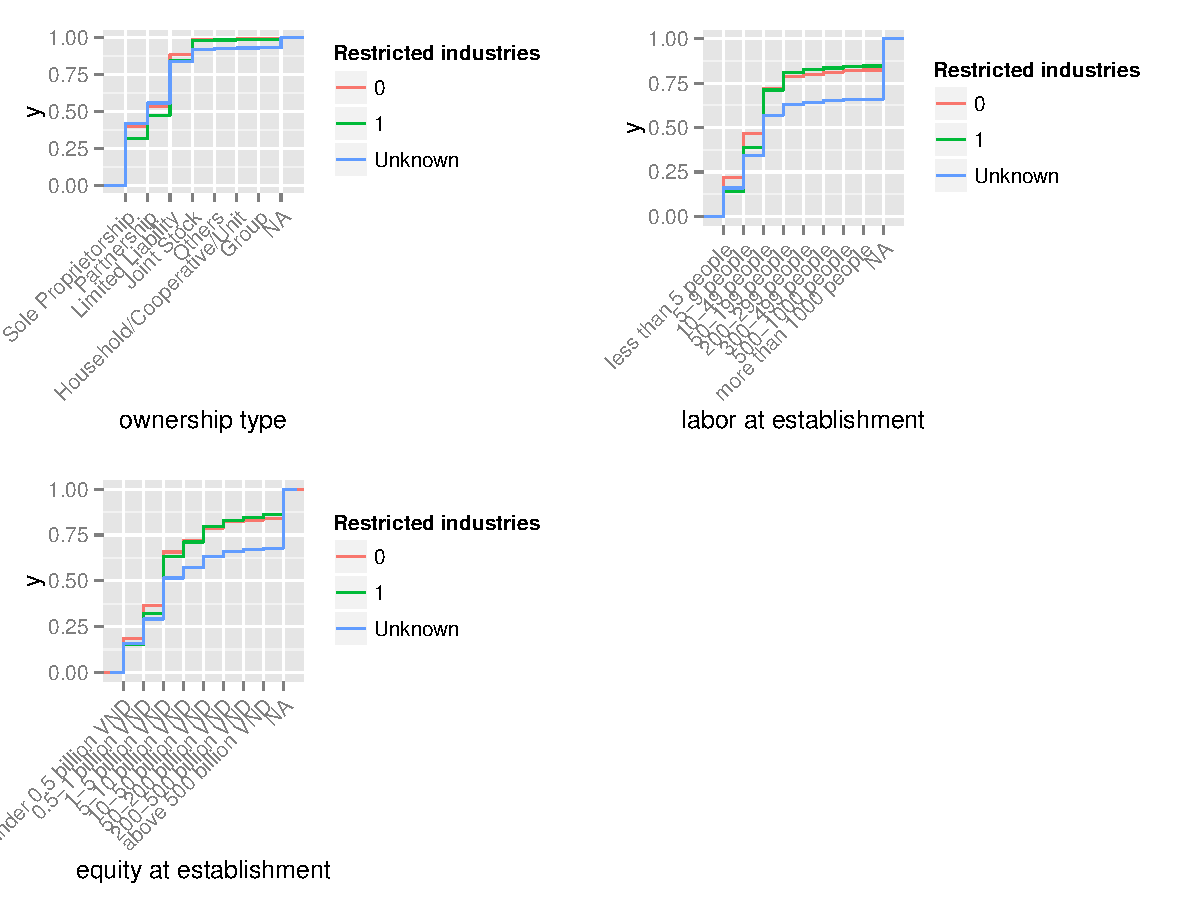
\includegraphics[width=\textwidth, height=\textheight,keepaspectratio]{../figure/by_restrict_owner-labor-equity}
\caption{The relationship between a province's FDI bias and attitude towards the private sector}
\label{fig:by_restrict_owner}
\end{figure}

\begin{figure}[!ht]
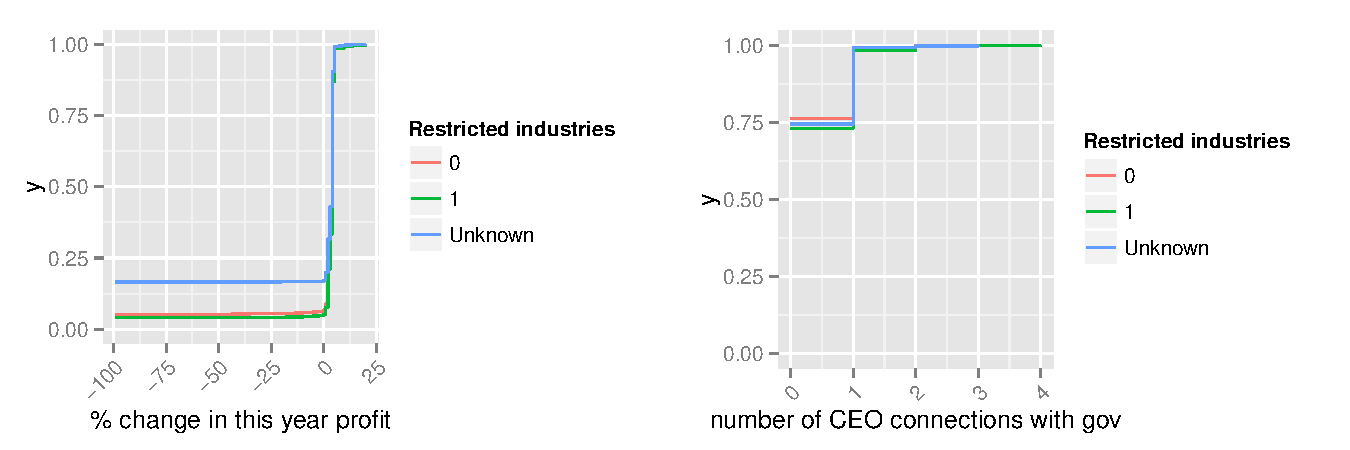
\includegraphics[width=\textwidth, height=\textheight,keepaspectratio]{../figure/by_restrict_performance-connection}
\caption{The relationship between a province's FDI bias and attitude towards the private sector}
\label{fig:by_restrict_performance}
\end{figure}

\subsection{Conjoint analysis}

The crucial causal mechanism in my theory is the utility calculation of provincial officials, which weighs between the developmental impact and the potential for corruption of FDI. It is difficult to fully examine this key step relying solely on observational data because what the officials truly want may not be fulfilled due to external factors and thus cannot be observed. Furthermore, what an official wants from a FDI firm is often hard to tease out completely. A big FDI firm is an attractive source of rent, but it also brings job and technology. Indeed, perhaps this high correlation is precisely why it is so easy for officials to extract rent from FDI under the guise of promoting economic development.

To truly get at the utility calculation of provincial officials, I plan to conduct a survey experiment using conjoint analysis to ask provincial officials about their preference between two hypothetical FDI firms \citep{Hainmueller2014}. The characteristics of these firms will be randomly varied across several dimensions: 1) industry, 2) size of labor force, 3) capital, 4) technology age, and 5) land, which proxies for corruption opportunities.

\subsubsection{Why choose land as a proxy for corruption?}

To discern the local officials' preference for corruption opportunity versus developmental impact, one must vary the hypothetical FDI projects along a characteristic that can only be attractive to officials because of its potential for corruption and not because of any other reasons. The amount of land a project requires is the best proxy for corruption in this regard. Since land is such a scarce resource with rapidly rising value in Vietnam, acquiring land from current tenants and farmers is a difficult, sometimes violent, process. Therefore, there is neither good developmental nor political reason for local officials to prefer a project that needs a large amount of land. In contrast, other characteristics of a FDI project can be preferred by officials for many different reasons. For example, a well capitalized project may signify a large pot of money to dip in, but it may also be attractive for the labor productivity enhancing effect of its capital. Similarly, a FDI firm with a large labor force may curry favor with officials to suppress their workers, but it may also be appealing for the jobs it creates. 

Unlike those factors, land is unambiguously an indication of corruption opportunities. With a high level of \textit{monopoly} and \textit{discretion}, local officials are able to sell land access, something that investors are eager to buy.

1) Monopolistic control over land supply: At the start of Vietnam's liberalization (under Land Law 1993), any exchange of land between land users and investors must go through the local government. Investors had to negotiate with all levels of local governments (i.e. commune, district, and province level people's committees) to acquire land---a complex process that encouraged investors to use informal procedures and fees to expedite. Importantly, the price of land was solely determined by the local government, which was usually 10-30\% of the market price. Therefore, officials were able to extract bribes with both their gate-keeping and price-setting powers over land.

Subsequent land law reforms (2003 and 2013) attempted to bring the land acquisition process closer to a market approach and lessen the monopolistic control of the local government over land. For example, Land Law 2003 specified two methods for investors to acquire lands: voluntary and compulsory. Under compulsory land acquisition (akin to eminent domain), local governments retain the power to acquire land with compensation then allocate to approved investors. Under the newly-introduced voluntary land acquisition, investors negotiate with and buy from land users in a private market transaction. Despite the option of buying lands from private users, in practice most investment projects tellingly opted for compulsory land acquisition by the state. With the local government's coercive power and legal ability to set compensation value on their side, investors find compulsory land acquisition both faster and cheaper, and thus worth paying for.

Similarly, despite many calls for removing the state's control over land, Land Law 2013 disappointed with its insistence on ``people's ownership'' of land instead of adopting a fully private ownership system. Furthermore, the law preserves the state's right to acquire land for the vaguely defined ``socioeconomic development'' and ``national interest,'' which expansively includes the development of industrial zones.

2) Discretionary allocation of land to selected investors: Opportunities for corruption also arise from two discretionary powers of the local governments. First, land acquired by the government is allocated directly to approved investors instead of through public auction, an option allowed by law but rarely practiced by local governments. Second, in many cases, local officials even modify the existing land use plans according to the suggestions of investors, making available land that was previously not zoned for business development. Without any standard guideline for investor approval, this process relies heavily on personal contacts and is prone to bribery and kickback.

An important symptom of this corrupt practice is the lack of transparency in the land allocation process and decision. Key information, such as the criteria of project approval, the shortlist of investors, the profile of the selected projects and investors, and the (dictated) price of land, are kept among selected investors and a few state officials involved. Even a straightforward compliance with transparency regulation, i.e. the public posting of investment site maps, is not fulfilled. In a 2010 study, DEPOCEN researchers could only access the investment site maps in 2 of the 12 visited provinces \citep{Anderson2011}.\footnote{But Land law 2013 does remove the direct allocation of land to approved project, instead try to increase the number of land auctions. Does this have an effect?}

\subsubsection{Conjoint analysis design}
Please read the following description carefully. Then, please indicate which project you prefer to grant investment license (cap giay phep dau tu).

\begin{center}
  \begin{tabular}{ c | c | c }
    \hline
     & Project 1 (Du an 1) & Project 2 (Du an 1) \\ \hline
    Industry &  &  \\ \hline
    Labor force &  &  \\ \hline
    Capital &  &  \\ \hline
    Land &  &  \\ \hline
    Technology age &  &  \\ \hline
    \hline
  \end{tabular}
\end{center}

If you have to choose, which project do you prefer to grant investment license? Project 1 / Project 2

\begin{itemize}
\item Industry: textile, electronics, automobile, consumer product
\item Labor force: 5, 50, 100, 200, 500 employees
\item Capital:
\item Land:
\item Technology age: 
\end{itemize}
